\documentclass[11pt, a4paper]{article}

\usepackage{graphicx}
\usepackage[english]{babel}
\usepackage[utf8x]{inputenc}
\usepackage{amsmath}
\usepackage[a4paper,top=3cm,bottom=2cm,left=2cm,right=2cm,marginparwidth=1.75cm]{geometry}
\usepackage{amssymb}

\graphicspath{ {./images} }

\makeatletter
\renewcommand*\env@matrix[1][*\c@MaxMatrixCols c]{%
  \hskip -\arraycolsep
  \let\@ifnextchar\new@ifnextchar
  \array{#1}}
\makeatother

\begin{document}
\setcounter{section}{5}

\section{Lecture 6 (27/02/2020)}
\subsection{Work and Energy}
\begin{equation}
  W = Fr\cos(\theta) = \int_{C}\vec{F}(\vec{r})\,d\vec{r}
\end{equation}
Work is a form of energy which is defined by displacement of mass
as a result of some force acting on an object. Only the component of the force
along the path the mass travels does actual work, which is represented by the $\cos(\theta)$ term.
There are several other forms of mechanical energy. These are as follows:
\begin{align}
  &E_{kin} = \frac{1}{2}mv^2 \qquad \text{Kinetic energy}\\
  &E_{pot} = mgh \qquad \text{Potential energy as heigt}\\
  &E_{pot} = \frac{1}{2}ks^2 \qquad \text{Potential energy stored in a spring}
\end{align}

\subsection{Conservative and non-conservative forces}
A force is defined to be conservative when the work as defined by equation (1) along any path
$C$ is only dependent on the beginning and ending point. An example of this is gravity.
The force of gravity always pulls mass to the earth in a straight line, thus the work done is only dependent
on the height at which the mass started. For a closed path this takes the following form:
\begin{equation}
  \oint \vec{F}(\vec{r})\,d\vec{r} = 0
\end{equation}
This basically means that the work done along any closed path must be equal to $0$
in order for a force to be conservative. A different way of formulating this can be found using
Stokes' Theorem\footnote{The exact method is irrelevant for now google it if interested}, which 
will give the following form:
\begin{equation}
  \nabla \times \vec{F}(\vec{r}) = 0
\end{equation}
Which basically means that the scalar field associated with the force does not rotate.

\subsection{Energy sums}
Energy sums are usually applied to systems where time is either an unknown or not
explicitly given or asked. The principle of an energy sum is just an application of the first law
of thermodynamics which states: \textit{Energy cannot be created nor destroyed, it can only be redirected.}
Because of this we know the following:
\begin{equation}
  E_{in} = E_{out}
\end{equation}
In the most general form this looks like the following:
\begin{equation}
  T_1 + V_1 + U = T_2 + V_2
\end{equation}
Where $T$ is the kinetic energy, $V$ is the total potential energy and 
$U$ is the work done. Rewriting this gives:
\begin{equation}
  \frac{1}{2}mv_1^2 + mgh_1 + \frac{1}{2}ks_1^2 + \int_{s_1}^{s_2}F\,ds = \frac{1}{2}ks_2^2 + mgh_2
\end{equation}

Suppose a ball is being thrown into the air with the inital velocity $v_1$. The energy sum would look like the following:
\begin{gather}
  \frac{1}{2}mv_1^2 = mgh_1\\
  h_2 = \frac{v_1^2}{2g}
\end{gather}
Equation (11) describes the height of the ball in terms of velocity. This would usually be done with the equation
of motion, solving for $t$ at $v=0$ and then filling that in after integrating a second time. This method is not explicitly dependent on time.

\subsection{Example with a spring}
\begin{figure}[h]
  \centerline{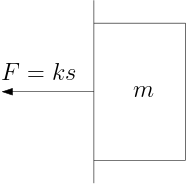
\includegraphics[width=40mm]{images/Spring.png}}
  \caption{The Free Body Diagram of the spring used for this example}
\end{figure}
\begin{gather}
  \Sigma F_x = -ks = ma\\
  a = \frac{-ks}{m}
\end{gather}
Since we know from an earlier lecture that $a\,ds = v\,dv$:
\begin{gather}
  -ks\,ds = mv\,dv\\
  \int_{s_1}^{s_2}-ks\,ds = \int_{v_1}^{v_2}mv\,dv\\
  -\frac{1}{2}ks^2 \Big|_{s_1}^{s_2} = \frac{1}{2}mv^2 \Big|_{v_1}^{v_2}\\
  -\frac{1}{2}ks_2^2 + \frac{1}{2}ks_1^2 = \frac{1}{2}mv_2^2 - \frac{1}{2}mv_1^2\\
  \frac{1}{2}ks_1^2 + \frac{1}{2}mv_1^2 = \frac{1}{2}ks_2^2 + \frac{1}{2}mv_2^2 \\
  T_1 + V_1 = T_2 + V_2
\end{gather}
Note that equation (18) and (19) are equivalant.
The important take away from this is the following:

\begin{equation}
  \int \Sigma F\,ds = \int ma\,ds = \int mv\,dv
\end{equation}

\end{document}